% =====================================================================
% Snippet: attention-heatmap.tex
% =====================================================================
% USAGE: Standalone demo of N×N attention heatmap with colorbar.
% Copy the tikzpicture content (lines marked with %% COPY-START / END)
% into your figure.tex, then replace placeholders:
%   - N: matrix size (default 6)
%   - cell_size: cell side in cm (default 0.5)
%   - label_prefix: row/col label letter (default "t")
%   - origin_x, origin_y: anchor position
%   - title: heatmap title (default "Attention Weights")
%
% The heatmap uses a diagonal-dominant pattern (alpha_ii > alpha_ij)
% which is realistic for self-attention. Adjust the formula on line 32
% to change the pattern.
% =====================================================================

\documentclass[tikz,border=10pt]{standalone}
\usepackage{xcolor,tikz}
\usetikzlibrary{positioning,calc}

% Light background (硬约束)
\definecolor{acaPurpleLine}{HTML}{6E3FA0}
\definecolor{acaPurpleFill}{HTML}{EDE3F6}
\definecolor{acaBlueLine}{HTML}{3060A8}
\definecolor{acaBlueFill}{HTML}{DCE6F4}
\definecolor{cellLo}{HTML}{F0E8F8}
\definecolor{cellHi}{HTML}{6E3FA0}

\begin{document}
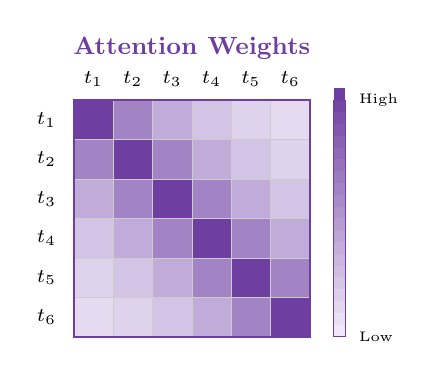
\begin{tikzpicture}

%% COPY-START =========================================================

% --- PARAMETERS (replace these) ---
\def\N{6}                % matrix size (rows × cols)
\def\cs{0.5}             % cell size in cm
\def\xO{0}               % origin x
\def\yO{0}               % origin y
\def\labpre{t}           % row/col label prefix (e.g., "t_1..t_N")

% --- HEATMAP CELLS ---
% Diagonal-dominant pattern: alpha_ij ∝ exp(-|i-j|/2) + small noise.
% Replace the formula `{(exp(-abs(\i-\j)/2)*100)}` with your data.
\foreach \i in {1,...,\N} {
  \foreach \j in {1,...,\N} {
    \pgfmathsetmacro\val{exp(-abs(\i-\j)/2)*100}
    \pgfmathsetmacro\val{int(\val)}
    \pgfmathsetmacro\cx{\xO + (\j - 0.5) * \cs}
    \pgfmathsetmacro\cy{\yO - (\i - 0.5) * \cs}
    \fill[cellHi!\val!cellLo]
      (\cx - \cs/2, \cy - \cs/2) rectangle (\cx + \cs/2, \cy + \cs/2);
  }
}

% --- GRID LINES ---
\draw[step=\cs cm, gray!40, very thin]
  (\xO, \yO) grid (\xO + \N*\cs, \yO - \N*\cs);
\draw[acaPurpleLine, line width=0.7pt]
  (\xO, \yO) rectangle (\xO + \N*\cs, \yO - \N*\cs);

% --- ROW LABELS (left of heatmap) ---
\foreach \i in {1,...,\N} {
  \pgfmathsetmacro\cy{\yO - (\i - 0.5) * \cs}
  \node[anchor=east, font=\scriptsize]
    at (\xO - 0.1, \cy) {$\labpre_{\i}$};
}

% --- COL LABELS (above heatmap) ---
\foreach \j in {1,...,\N} {
  \pgfmathsetmacro\cx{\xO + (\j - 0.5) * \cs}
  \node[anchor=south, font=\scriptsize]
    at (\cx, \yO + 0.05) {$\labpre_{\j}$};
}

% --- TITLE ---
\node[anchor=south, font=\small\bfseries, color=acaPurpleLine]
  at (\xO + \N*\cs/2, \yO + 0.4) {Attention Weights};

% --- COLORBAR (right side) ---
\pgfmathsetmacro\cbX{\xO + \N*\cs + 0.3}
\pgfmathsetmacro\cbW{0.15}
\pgfmathsetmacro\cbH{\N*\cs}
\foreach \t in {0,5,...,100} {
  \pgfmathsetmacro\ty{\yO - \cbH + \cbH * \t / 100}
  \pgfmathsetmacro\tyN{\yO - \cbH + \cbH * (\t+5) / 100}
  \fill[cellHi!\t!cellLo]
    (\cbX, \ty) rectangle (\cbX + \cbW, \tyN);
}
\draw[acaPurpleLine, line width=0.5pt]
  (\cbX, \yO - \cbH) rectangle (\cbX + \cbW, \yO);
\node[anchor=west, font=\tiny] at (\cbX + \cbW + 0.05, \yO) {High};
\node[anchor=west, font=\tiny] at (\cbX + \cbW + 0.05, \yO - \cbH) {Low};

%% COPY-END ===========================================================

\end{tikzpicture}
\end{document}
